\documentclass[5p,sort&compress]{elsarticle}

\usepackage{amssymb}    % Mathematical symbols
\usepackage{amsmath}    % More options for mathematics
\usepackage{subfigure}  % More options for figures
\usepackage{epstopdf}   % Convert eps to pdf
\usepackage[separate-uncertainty=true]{siunitx}   % Proper formatting of units in math mode
\usepackage{color}      % Supports text color if needed
\usepackage{soul}       % https://ctan.org/pkg/soul
\usepackage{lmodern}    % Loading fonts
\usepackage{hyperref}   % To insert clickable references/urls
\usepackage{listings}   % To input code in the text
\usepackage{amsmath}
\usepackage{amsmath}
\usepackage{amssymb}
\usepackage{graphicx}
\usepackage{epstopdf}
\usepackage{booktabs}
\setlength{\parskip}{2em}
\newcommand{\stirlingii}{\genfrac{\{}{\}}{0pt}{}}

% Choose the style of the reference list (do not change)
\bibliographystyle{elsarticle-num}

\journal{ifding/learning-notes}

% Begin the document

\begin{document}

\begin{frontmatter}
    \title{Chatper 2: Probability Distributions}
    \author{ifding}
    
    \begin{abstract}
        Binary Variables, Multinomial Variables, Gaussian Distribution, Exponential Family, Nonparametric Methods
    \end{abstract}


\end{frontmatter}

%% How to make a heading and divide the documents into different sections

\textit{density estimation}:  model the probability distribution $p(x)$ of a random variable $x$, given a finite set $x_1, \ldots, x_N$ of observations. It should be emphasized that the problem of density estimation is \textbf{fundamentally ill-posed}, because there infinitely probability distributions that could have given rise to the observed finite data set. Indeed, any distribution $p(x)$ that is nonzero at each of the data points $x_1, \ldots, x_N$ is a potential candidate.

\textit{parametric} distributions, e.g., binomial and multinomial distributions for discrete random variables and Gaussian distribution for continuous random variables, are governed by a small number of adaptive parameters, such as mean and variance in a Gaussian.

\textit{nonparametric} density estimation methods: the distribution typically depends on the size of the data set. Such models still contain parameters, but these control the model complexity rather than the form of the distribution.


\section{Binary Variables}

Considering a binary random variable $x \in \{0, 1\}$ The probability of $x=1$ will be denoted by the parameter $\mu$, so that $p(x=1 | \mu) = \mu$, where $0 \leq \mu \leq 1$, $p(x=0 | \mu) = 1- \mu$. The \textit{Bernoulli} distribution:
\begin{equation}
\operatorname{Bern}(x | \mu)=\mu^{x}(1-\mu)^{1-x}
\end{equation}
\begin{equation}
\begin{aligned} \mathbb{E}[x] &=\mu \\ \operatorname{var}[x] &=\mu(1-\mu) \end{aligned}
\end{equation}

Suppose we have a data set $\mathcal{D} = \{x_1, \ldots, x_N\}$, which are drawn independently from $p(x|\mu)$, the likelihood function:
\begin{equation}
p(\mathcal{D} | \mu)=\prod_{n=1}^{N} p\left(x_{n} | \mu\right)=\prod_{n=1}^{N} \mu^{x_{n}}(1-\mu)^{1-x_{n}}
\end{equation}

\begin{equation}
\begin{aligned}
\ln p(\mathcal{D} | \mu)=\sum_{n=1}^{N} \ln p\left(x_{n} | \mu\right) &= \\ \sum_{n=1}^{N}\left\{x_{n} \ln \mu+\left(1-x_{n}\right) \ln (1-\mu)\right\}
\end{aligned}
\end{equation}

The log likelihood function depends on the N observations $x_n$ only through their sum $\sum_n x_n$, which provides an example of a \textit{sufficient statistic} for the data under this distribution. If set the derivative of $\ln{p(\mathcal{D}|\mu)}$ with respect to $\mu$ equal to zero,
\begin{equation}
\mu_{\mathrm{ML}}=\frac{1}{N} \sum_{n=1}^{N} x_{n}
\end{equation}
which is known as the \textit{sample mean}. If we denote the number of observations of $x=1$ (heads) within this data set by $m$, then $\mu_{\mathrm{ML}}=m/N$. Suppose we flip a coin 3 times and happen to observe 3 heads. Then $N=m=3$ and $\mu_{\mathrm{ML}}=1$. In this case, the maximum likelihood result would predict that all future observations should give heads. This is an extreme example of the over-fitting associated with maximum likelihood.

The \textit{binomial} distribution. To obtain the normalization coefficient, we have to add up all of the possible ways of obtaining m heads.
\begin{equation}
\begin{aligned} \operatorname{Bin}(m | N, \mu) &=\left(\begin{array}{c}{N} \\ {m}\end{array}\right) \mu^{m}(1-\mu)^{N-m} \\\left(\begin{array}{c}{N} \\ {m}\end{array}\right) & \equiv \frac{N !}{(N-m) ! m !} \end{aligned}
\end{equation}


\section{Multinomial Variables}

1-of-K scheme: K-dimensional vector \textbf{x} in which one of the elements $x_k$ equals 1, and all remaining elements equal 0. For example, $K=6$ and $x_3 =1 $, then
\begin{equation}
    \mathbf{x} = (0, 0, 1, 0, 0)^T.
\end{equation}
Note that such vectors satisfy $\sum_{k=1}^K x_k =1$. If we denote the probability of $x_k=1$ by the parameter $\mu_k$, then the distribution of $\mathbf{x}$ is given
\begin{equation}
p(\mathbf{x} | \boldsymbol{\mu})=\prod_{k=1}^{K} \mu_{k}^{x_{k}}
\end{equation}
where $\boldsymbol{\mu} = (\mu_1, \ldots, \mu_K)^T$, and the parameters $\mu_k$ are constrained to satisfy $\mu_k \geq 0$ and $\sum_k \mu_k =1$, because they represent probabilities. The distribution $p(\mathbf{x} | \boldsymbol{\mu})$ can be regarded as a generalization of Bernoulli distribution to more than two outcomes. It's easily seen that the distribution is normalized
\begin{equation}
\begin{aligned}{\sum_{\mathbf{x}} p(\mathbf{x} | \boldsymbol{\mu})=\sum_{k=1}^{K} \mu_{k}=1} \\ {\mathbb{E}[\mathbf{x} | \boldsymbol{\mu}]=\sum_{\mathbf{x}} p(\mathbf{x} | \boldsymbol{\mu}) \mathbf{x}=\left(\mu_{1}, \ldots, \mu_{M}\right)^{\mathrm{T}}=\boldsymbol{\mu}}\end{aligned}
\end{equation}


\section{The Gaussian Distribution}
It's widely used model for the distribution of continuous variables. In the case of a single variable $x$,
\begin{equation}
\mathcal{N}\left(x | \mu, \sigma^{2}\right)=\frac{1}{\left(2 \pi \sigma^{2}\right)^{1 / 2}} \exp \left\{-\frac{1}{2 \sigma^{2}}(x-\mu)^{2}\right\}
\end{equation}
where $\mu$ is the mean and $\sigma^2$ is the variance. For a $D$-dimensional vector $\boldsymbol{x}$, the multivariate Gaussian distribution $\mathcal{N}(\mathbf{x} | \boldsymbol{\mu}, \mathbf{\Sigma}) = $
\begin{equation}
 \frac{1}{(2 \pi)^{D / 2}} \frac{1}{|\mathbf{\Sigma}|^{1 / 2}} \exp \left\{-\frac{1}{2}(\mathbf{x}-\boldsymbol{\mu})^{\mathrm{T}} \mathbf{\Sigma}^{-1}(\mathbf{x}-\boldsymbol{\mu})\right\}
\end{equation}
where $\mu$ is a $D$-dimensional mean vector, $\mathbf{\Sigma}$ is $D \times D$ covariance matrix, and $|\mathbf{\Sigma}|$ denotes the determinant of $\mathbf{\Sigma}$.

The \textit{central limit theorem}, considering $N$ variables $x_1$, $\ldots$, $x_N$ each of which has a uniform distribution over the interval [0,1] and then considering the distribution of the mean $(x_1 + \ldots + x_N)/N$. For large $N$, this distribution tends to a Gaussian.

The functional dependence of the Gaussian on $\boldsymbol{x}$ is through the quadratic form
\begin{equation}
\Delta^{2}=(\mathbf{x}-\boldsymbol{\mu})^{\mathrm{T}} \mathbf{\Sigma}^{-1}(\mathbf{x}-\boldsymbol{\mu})
\end{equation}
which appears in the exponent. The quantity $\Delta$ is called the \textit{Mahalanobis distance} from $\boldsymbol{\mu}$ to $\boldsymbol{x}$ and reduces to the Euclidean distance when $\mathbf{\Sigma}$ is the identity matrix.

First of all, the matrix $\mathbf{\Sigma}$ can be taken to be symmetric, without loss of generality. Now consider the eigenvector equation for the covariance matrix
\begin{equation}
\boldsymbol{\Sigma} \mathbf{u}_{i}=\lambda_{i} \mathbf{u}_{i}
\end{equation}
where $i = 1, \ldots, D$. Because $\mathbf{\Sigma}$ is real, symmetric matrix its eigenvalues will be real, and its eigenvectors can be chosen to form an orthonormal set
\begin{equation}
\mathbf{u}_{i}^{\mathrm{T}} \mathbf{u}_{j}=I_{i j}
\end{equation}
where $I_{ij}$ is the i, j element of the identify matrix and satisfies
\begin{equation}
I_{i j}=\left\{\begin{array}{ll}{1,} & {\text { if } i=j} \\ {0,} & {\text { otherwise }}\end{array}\right.
\end{equation}
$\mathbf{\Sigma}$ and $\mathbf{\Sigma}^{-1}$ can be expressed as
\begin{equation}
\begin{aligned} \boldsymbol{\Sigma} &=\sum_{i=1}^{D} \lambda_{i} \mathbf{u}_{i} \mathbf{u}_{i}^{\mathrm{T}} \\
\boldsymbol{\Sigma}^{-1} &=\sum_{i=1}^{D} \frac{1}{\lambda_{i}} \mathbf{u}_{i} \mathbf{u}_{i}^{\mathrm{T}} \end{aligned}
\end{equation}

The quadratic form becomes
\begin{equation}\label{eqn:quadratic}
\begin{aligned}{\Delta^{2}=\sum_{i=1}^{D} \frac{y_{i}^{2}}{\lambda_{i}}} \\ {y_{i}=\mathbf{u}_{i}^{\mathrm{T}}(\mathbf{x}-\boldsymbol{\mu})}\end{aligned}
\end{equation}
We can interpret ${y_i}$ as a new coordinate system defined by the orthonormal vectors $\boldsymbol{\mu}_i$ that are shifted and rotated with respect to the original $x_i$ coordinates. Forming the vector $\boldsymbol{y} = (y_1, \ldots, y_D)^T$, we have
\begin{equation}
\mathbf{y}=\mathbf{U}(\mathbf{x}-\boldsymbol{\mu})
\end{equation}
where $\mathbf{U}$ is a matrix whose rows are given by $\mathbf{u}_{i}^{\mathrm{T}}$. It's an orthogonal matrix, i.e., it satisfies $\mathbf{U}\mathbf{U}^{\mathrm{T}} = \mathbf{I}$, and here also $\mathbf{U}^{\mathrm{T}} \mathbf{U} = \mathbf{I}$, where $\mathbf{I}$ is the identity matrix.

The quadratic form, and hence the Gaussian density, will be constant on surfaces for which Equation~\ref{eqn:quadratic} is constant. As illustrated in Figure~\ref{fig:2.7}, a Gaussian in a two-dimensional space $\boldsymbol{x} = (x_1, x_2)$ is exp(-1/2) of its value at $\boldsymbol{x} = \boldsymbol{\mu}$. The major axes of the ellipse are defined by the eigenvectors $\boldsymbol{u}_i$ of the covariance matrix, with corresponding eigenvalues $\lambda_i$.

\begin{figure}[ht]
     \centering
     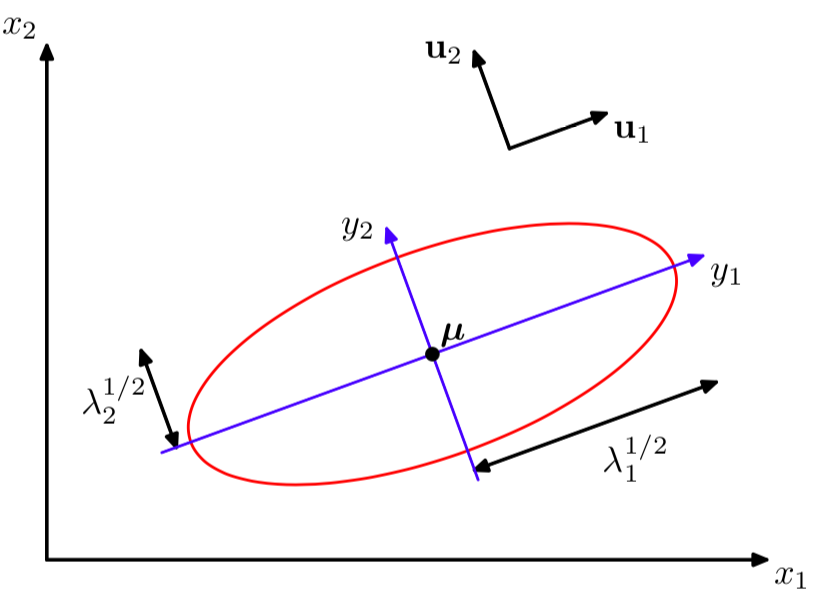
\includegraphics[width = \linewidth]{figure/fig2-7.png}
     \caption{The red curve shows the elliptical surface of constant probability density for a Gaussian in a two-dimensional space.}
     \label{fig:2.7}
\end{figure}

Now consider the form of the Gaussian distribution in the new coordinate system defined by the $y_i$, a Jacobian matrix $\mathbf{J}$ with elements given by
\begin{equation}
J_{i j}=\frac{\partial x_{i}}{\partial y_{j}}=U_{j i}
\end{equation}
where $U_{j i}$ are the elements of the matrix $\mathbf{U}^{\mathrm{T}}$.
\begin{equation}
|\mathbf{J}|^{2}=\left|\mathbf{U}^{\mathrm{T}}\right|^{2}=\left|\mathbf{U}^{\mathrm{T}}\right||\mathbf{U}|=\left|\mathbf{U}^{\mathrm{T}} \mathbf{U}\right|=|\mathbf{I}|=1
\end{equation}
and hence $|\mathbf{U}| = 1$. The determinant $|\mathbf{\Sigma}|$ of the covariance matrix can be written as the product of its eigenvalues, and hence
\begin{equation}
|\boldsymbol{\Sigma}|^{1 / 2}=\prod_{j=1}^{D} \lambda_{j}^{1 / 2}
\end{equation}
Thus in the $y_j$ coordinate system, the Gaussian distribution takes the form
\begin{equation}
p(\mathbf{y})=p(\mathbf{x})|\mathbf{J}|=\prod_{j=1}^{D} \frac{1}{\left(2 \pi \lambda_{j}\right)^{1 / 2}} \exp \left\{-\frac{y_{j}^{2}}{2 \lambda_{j}}\right\}
\end{equation}
which is the product of $D$ independent univariate Gaussian distributions. The eigenvectors therefore define a new set of shifted and rotated coordinates with respect to which \textbf{the joint probability distribution factorizes into a product of independent distributions}. The integral of the distribution in the $\boldsymbol{y}$ coordinate system is then
\begin{equation}
\int p(\mathbf{y}) \mathrm{d} \mathbf{y}=\prod_{j=1}^{D} \int_{-\infty}^{\infty} \frac{1}{\left(2 \pi \lambda_{j}\right)^{1 / 2}} \exp \left\{-\frac{y_{j}^{2}}{2 \lambda_{j}}\right\} \mathrm{d} y_{j}=1
\end{equation}
This confirms that the multivariate Gaussian is indeed normalized.

\begin{equation}
\begin{aligned}
\mathbb{E}[\mathbf{x}]=\boldsymbol{\mu} \\
\mathbb{E}\left[\mathbf{x} \mathbf{x}^{\mathrm{T}}\right]=\boldsymbol{\mu} \boldsymbol{\mu}^{\mathrm{T}}+\mathbf{\Sigma} \\
\operatorname{cov}[\mathbf{x}]=\mathbb{E}[(\mathbf{x}-\mathbb{E}[\mathbf{x}])(\mathbf{x}-\mathbb{E}[\mathbf{x}])^{\mathrm{T}}] = \mathbf{\Sigma}
\end{aligned}
\end{equation}

Consider the number of free parameters in the distribution. A general symmetric covariance matrix $\mathbf{\Sigma}$ will have $D(D+1)/2$ independent parameters, and there are another $D$ independent parameters in $\boldsymbol{\mu}$, giving $D(D+3)/2$ parameters in total. For large $D$, the computation is expensive. One way is to use restricted forms of the covariance matrix. \textit{diagonal} covariance matrices, so that $\mathbf{\Sigma} = \operatorname{diag}(\sigma_i^2)$, we then have a total of $2D$ independent parameters in the density model. We could further restrict the covariance matrix to be proportional to the identity matrix, $\mathbf{\Sigma} = \sigma^2\mathbf{I}$, known as an \textit{isotropic covariance}, giving $D+1$ independent parameters in the model.

\begin{figure}[ht]
     \centering
     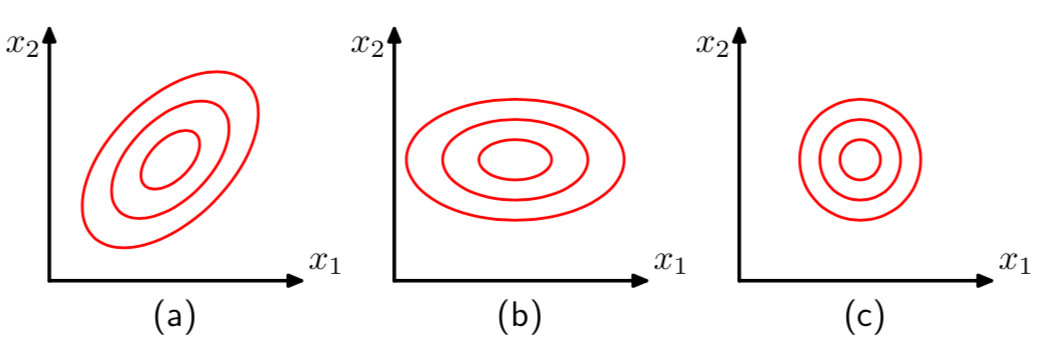
\includegraphics[width = \linewidth]{figure/fig2-8.png}
     \caption{Contours of constant probability density for a Gaussian distribution in which the covariance matrix is (a) of general form, (b) diagonal, agligned with the coordinate axes, and (c), concentric circles.}
     \label{fig:2.8}
\end{figure}

The three possibilities of general, diagonal, and isotropic covariance matrices are illustrated in Figure~\ref{fig:2.8}. Such approaches limit the number of degrees of freedom and make inversion of the covariance matrix a much faster operation, but they also greatly restrict the form of the probability density and limit its ability to capture interesting correlations in the data. A further limitation of the Gaussian distribution is that it is intrinsically unimodal (i.e., has a single maximum) and so is unable to provide a good approximation to multimodal distributions.



\subsection{Conditional Gaussian distributions}


An important property of the multivariate Gaussian distribution is that if two sets of variables are jointly Gaussian, then the conditional distribution of one set conditioned on the other is Gaussian, the marginal distribution of either set is also Gaussian.

Suppose $\boldsymbol{x}$ is a $D$-dimensional vector with Gaussian distribution $\mathcal{N}(\boldsymbol{x} | \boldsymbol{\mu}, \boldsymbol{\Sigma})$ and that we partition $\boldsymbol{x}$ into two disjoint subsets $\boldsymbol{x}_a$ and $\boldsymbol{x}_b$, $\boldsymbol{x}_a$ includes the first M components of $\boldsymbol{x}$, and $\boldsymbol{x}_b$ comprises the remaining $D-M$ components.
\begin{equation}
\boldsymbol{x}=\left(\begin{array}{l}{\boldsymbol{x}_{a}} \\ {\boldsymbol{x}_{b}}\end{array}\right)
\end{equation}
The mean vector $\mu$
\begin{equation}
\boldsymbol{\mu}=\left(\begin{array}{l}{\boldsymbol{\mu}_{a}} \\ {\boldsymbol{\mu}_{b}}\end{array}\right)
\end{equation}
and the covariance matrix
\begin{equation}
\boldsymbol{\Sigma}=\left(\begin{array}{cc}{\boldsymbol{\Sigma}_{a a}} & {\boldsymbol{\Sigma}_{a b}} \\ {\boldsymbol{\Sigma}_{b a}} & {\boldsymbol{\Sigma}_{b b}}\end{array}\right)
\end{equation}
Note that the symmetry $\boldsymbol{\Sigma}^{\mathrm{T}}=\boldsymbol{\Sigma}$, $\boldsymbol{\Sigma}_{aa}$ and $\boldsymbol{\Sigma}_{bb}$ are symmetric, $\boldsymbol{\Sigma}_{ba}=\boldsymbol{\Sigma}_{ab}^{\mathrm{T}}$.
\begin{equation}
\begin{aligned} \boldsymbol{\mu}_{a | b} &=\boldsymbol{\mu}_{a}+\boldsymbol{\Sigma}_{a b} \boldsymbol{\Sigma}_{b b}^{-1}\left(\mathbf{x}_{b}-\boldsymbol{\mu}_{b}\right) \\ \boldsymbol{\Sigma}_{a | b} &=\boldsymbol{\Sigma}_{a a}-\boldsymbol{\Sigma}_{a b} \boldsymbol{\Sigma}_{b b}^{-1} \boldsymbol{\Sigma}_{b a} \end{aligned}
\end{equation}
Note that the mean of the conditional distribution $p(x_a|x_b)$ is a linear function of $\boldsymbol{x}_b$ and that the covariance is independent of $\boldsymbol{x}_a$. This represents an example of a \textit{linear-Gaussian} model.

\begin{figure}
     \centering
     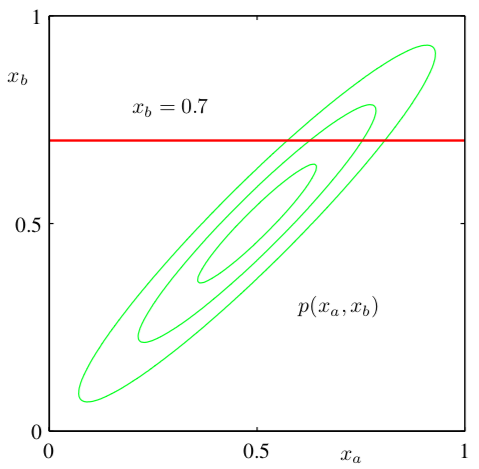
\includegraphics[width = \linewidth]{figure/fig2-9-1.png}
     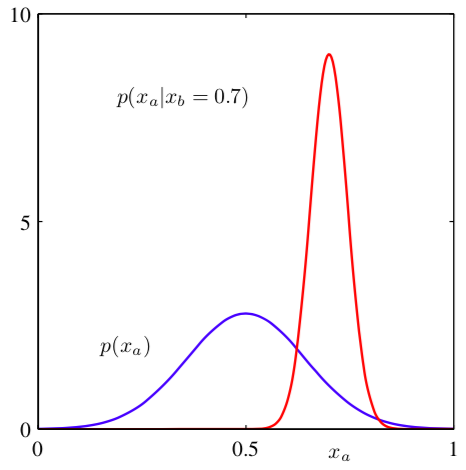
\includegraphics[width = \linewidth]{figure/fig2-9-2.png}     
     \caption{The plot on the top shows the contours of a Gaussian distribution $p(x_a, x_b)$ over two variables, and the plot on the bottom shows the marginal distribution $p(x_a)$ (blue curve) and the conditional distribution $p(x_a | x_b)$ for $x_b = 0.7$ (red curve).}
     \label{fig:2.9}
\end{figure}


\subsection{Marginal Gaussian distributions}

The marginal distribution given of 
\begin{equation}
p\left(\mathbf{x}_{a}\right)=\int p\left(\mathbf{x}_{a}, \mathbf{x}_{b}\right) \mathrm{d} \mathbf{x}_{b}
\end{equation}
which is also Gaussian. Efficient evaluation will be to identify the mean and covariance of the marginal distribution $p(\textbf{x}_a)$
\begin{equation}
\begin{aligned} \mathbb{E}\left[\mathbf{x}_{a}\right] &=\boldsymbol{\mu}_{a} \\ \operatorname{cov}\left[\mathbf{x}_{a}\right] &=\boldsymbol{\Sigma}_{a a} \end{aligned}
\end{equation}
\begin{equation}
p\left(\mathbf{x}_{a}\right)=\mathcal{N}\left(\mathbf{x}_{a} | \boldsymbol{\mu}_{a}, \mathbf{\Sigma}_{a a}\right)
\end{equation}

The conditional and marginal distributions associated with
a multivariate Gaussian involving two variables are shown in Figure~\ref{fig:2.9}.

\subsection{Maximum likelihood for the Gaussian}

Given a data set $\boldsymbol{X} = (\boldsymbol{x}_1, \ldots, \boldsymbol{x}_N)^T$ in which the observations $\{\boldsymbol{x}_n\}$ are assumed to be drawn independently from a multivariate Gaussian distribution. The log likelihood function is given by $\ln p(\mathbf{X} | \boldsymbol{\mu}, \mathbf{\Sigma}) = $
\begin{equation}
-\frac{N D}{2} \ln (2 \pi) -\frac{N}{2} \ln |\mathbf{\Sigma}|-\frac{1}{2} \sum_{n=1}^{N}\left(\mathbf{x}_{n}-\boldsymbol{\mu}\right)^{\mathrm{T}} \mathbf{\Sigma}^{-1}\left(\mathbf{x}_{n}-\boldsymbol{\mu}\right)
\end{equation}

The derivative of the log likelihood with respect to $\mu$ is given by
\begin{equation}
\frac{\partial}{\partial \boldsymbol{\mu}} \ln p(\mathbf{X} | \boldsymbol{\mu}, \mathbf{\Sigma})=\sum_{n=1}^{N} \boldsymbol{\Sigma}^{-1}\left(\mathbf{x}_{n}-\boldsymbol{\mu}\right)
\end{equation}
and setting this derivative to zero, the maximum likelihood estimate of the mean given by
\begin{equation}
\boldsymbol{\mu}_{\mathrm{ML}}=\frac{1}{N} \sum_{n=1}^{N} \mathbf{x}_{n}
\end{equation}
\begin{equation}
\mathbf{\Sigma}_{\mathrm{ML}}=\frac{1}{N} \sum_{n=1}^{N}\left(\mathrm{x}_{n}-\boldsymbol{\mu}_{\mathrm{ML}}\right)\left(\mathbf{x}_{n}-\boldsymbol{\mu}_{\mathrm{ML}}\right)^{\mathrm{T}}
\end{equation}
which involves $\mathbf{\Sigma}_{\mathrm{ML}}$ because this is the result of a joint maximization with respect to $\boldsymbol{\mu}$ and $\mathbf{\Sigma}$.
\begin{equation}
\begin{aligned} \mathbb{E}\left[\boldsymbol{\mu}_{\mathrm{ML}}\right] &=\boldsymbol{\mu} \\ \mathbb{E}\left[\boldsymbol{\Sigma}_{\mathrm{ML}}\right] &=\frac{N-1}{N} \boldsymbol{\Sigma} \end{aligned}
\end{equation}

The expectation of the maximum likelihood estimate for the mean is equal to the true mean. However, the maximum likelihood estimate for the covariance has an expectation that is less than the true value, and hence it is biased.

\subsection{Bayesian inference for the Gaussian}

The maximum likelihood framework gave point estimates for the parameters $\boldsymbol{\mu}$ and $\mathbf{\Sigma}$. Given a set of N observations $\boldsymbol{X}$, we suppose that the variance $\sigma^2$ is known, and consider the task of inferring the mean $\mu$.
\begin{equation}
\begin{aligned}
p(\mathbf{X} | \mu)=\prod_{n=1}^{N} p\left(x_{n} | \mu\right) & =  \\
\frac{1}{\left(2 \pi \sigma^{2}\right)^{N / 2}} \exp \left\{-\frac{1}{2 \sigma^{2}} \sum_{n=1}^{N}\left(x_{n}-\mu\right)^{2}\right\}
\end{aligned}
\end{equation}
Note that $p(\boldsymbol{X}|\mu)$ is not probability distribution over $\mu$ and is not normalized.

If we choose a prior $p(\mu)$ given by a Gaussian, it will be a conjugate distribution for this likelihood function. 
\begin{equation}
p(\mu) =\mathcal{N}\left(\mu | \mu_{0}, \sigma_{0}^{2}\right)
\end{equation}
and the posterior distribution is given by
\begin{equation}
p(\mu | \mathbf{X}) \propto p(\mathbf{X} | \mu) p(\mu) 
\end{equation}
\begin{equation}
\begin{array}{l}{~~~~~\qquad p(\mu | \mathbf{X})=\mathcal{N}\left(\mu | \mu_{N}, \sigma_{N}^{2}\right)} \\ {\text { where }} \\ {\qquad \begin{aligned} \mu_{N} &=\frac{\sigma^{2}}{N \sigma_{0}^{2}+\sigma^{2}} \mu_{0}+\frac{N \sigma_{0}^{2}}{N \sigma_{0}^{2}+\sigma^{2}} \mu_{\mathrm{ML}} \\ \frac{1}{\sigma_{N}^{2}} &=\frac{1}{\sigma_{0}^{2}}+\frac{N}{\sigma^{2}} \end{aligned}}\end{array}
\end{equation}

Now let us suppose that the mean is known and we wish to infer the variance. It turns out to be most convenient to work with the precision $\lambda \equiv 1/\sigma^2$. The likelihood function for $\lambda$ takes the form $p(\mathbf{X} | \lambda)=$
\begin{equation}\label{eqn:pxl}
\prod_{n=1}^{N} \mathcal{N}\left(x_{n} | \mu, \lambda^{-1}\right) \propto \lambda^{N / 2} \exp \left\{-\frac{\lambda}{2} \sum_{n=1}^{N}\left(x_{n}-\mu\right)^{2}\right\}
\end{equation}

This corresponds to the \textit{gamma} distribution which is defined by 
\begin{equation}
\operatorname{Gam}(\lambda | a, b)=\frac{1}{\Gamma(a)} b^{a} \lambda^{a-1} \exp (-b \lambda)
\end{equation}
The gamma distribution has a finite integral if $a > 0$, and the distribution itself is finite if $a \geq 1$. The mean and variance of the gamma distribution are given by
\begin{equation}
\begin{aligned} \mathbb{E}[\lambda] &=\frac{a}{b} \\ \operatorname{var}[\lambda] &=\frac{a}{b^{2}} \end{aligned}
\end{equation}

Consider a prior distribution Gam($\lambda|a_0, b_0$). If we multiply by the likelihood function (\ref{eqn:pxl}), then we obtain a posterior distribution
\begin{equation}
p(\lambda | \mathbf{X}) \propto \lambda^{a_{0}-1} \lambda^{N / 2} \exp \left\{-b_{0} \lambda-\frac{\lambda}{2} \sum_{n=1}^{N}\left(x_{n}-\mu\right)^{2}\right\}
\end{equation}
which we recognize as a gamma distribution of the form Gam($\lambda|a_N, b_N$) where
\begin{equation}
\begin{aligned}{a_{N}=a_{0}+\frac{N}{2}} \\ {b_{N}=b_{0}+\frac{1}{2} \sum_{n=1}^{N}\left(x_{n}-\mu\right)^{2}=b_{0}+\frac{N}{2} \sigma_{\mathrm{ML}}^{2}}\end{aligned}
\end{equation}
where $\sigma_{\mathrm{ML}}^2$ is the maximum likelihood estimator of the variance.


\subsection{Student's t-distribution}

If we have a univariate Gaussian $\mathcal{N}(x|\mu, \tau^{-1})$ together with a Gamma prior Gam($\tau | a, b$) and we integrate out the precision, we obtain the marginal distribution of x in the form 
\begin{equation}\label{eqn:t-distribution}
\begin{aligned} p(x | \mu, a, b) & \\ =\int_{0}^{\infty} \mathcal{N}\left(x | \mu, \tau^{-1}\right) \operatorname{Gam}(\tau | a, b) \mathrm{d} \tau & \\ = \int_{0}^{\infty} \frac{b^{a} e^{(-b \tau)} \tau^{a-1}}{\Gamma(a)}\left(\frac{\tau}{2 \pi}\right)^{1 / 2} \exp \left\{-\frac{\tau}{2}(x-\mu)^{2}\right\} \mathrm{d} \tau  & \\ =  \frac{b^{a}}{\Gamma(a)}\left(\frac{1}{2 \pi}\right)^{1 / 2}\left[b+\frac{(x-\mu)^{2}}{2}\right]^{-a-1 / 2} \Gamma(a+1 / 2) \end{aligned}
\end{equation}
By convention we define new parameters given by $\nu=2a$ and $\lambda=a/b$, in terms of which the distribution $p(x|\mu,\lambda,\nu)$ takes the form
\begin{equation}
\begin{aligned}
\operatorname{St}(x | \mu, \lambda, \nu) & = \\ \frac{\Gamma(\nu / 2+1 / 2)}{\Gamma(\nu / 2)}\left(\frac{\lambda}{\pi \nu}\right)^{1 / 2}\left[1+\frac{\lambda(x-\mu)^{2}}{\nu}\right]^{-\nu / 2-1 / 2}
\end{aligned}
\end{equation}
which is known as \textit{Student's t-distribution}. The parameter $\lambda$ is sometimes called the \textit{precision} of the t-distribution, the parameters $\nu$ is called the \textit{degrees of freedom}.

From (\ref{eqn:t-distribution}), we see that Student's t-distribution is obtained by adding up an infinite number of Gaussian distributions having the same mean but different precisions. This can be interpreted as an infinite mixture of Gaussians. This gives the t-distribution an important property called \textit{robustness}, which means that it's much less sensitive than the Gaussian to the presence of a few data points which are \textit{outliers}, as was seen in Figure~\ref{fig:2.16}.

\begin{figure}
     \centering
     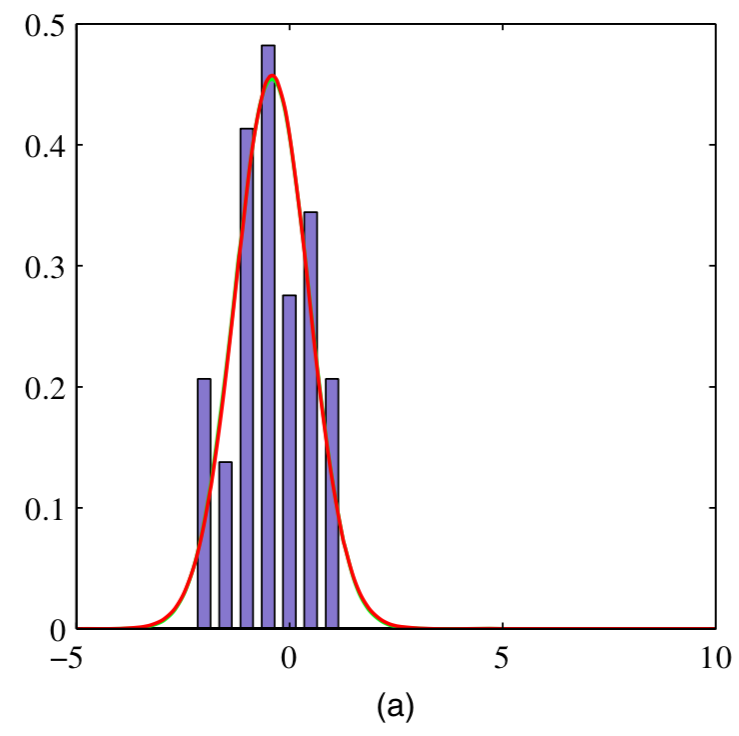
\includegraphics[width = \linewidth]{figure/fig2-16-1.png}
     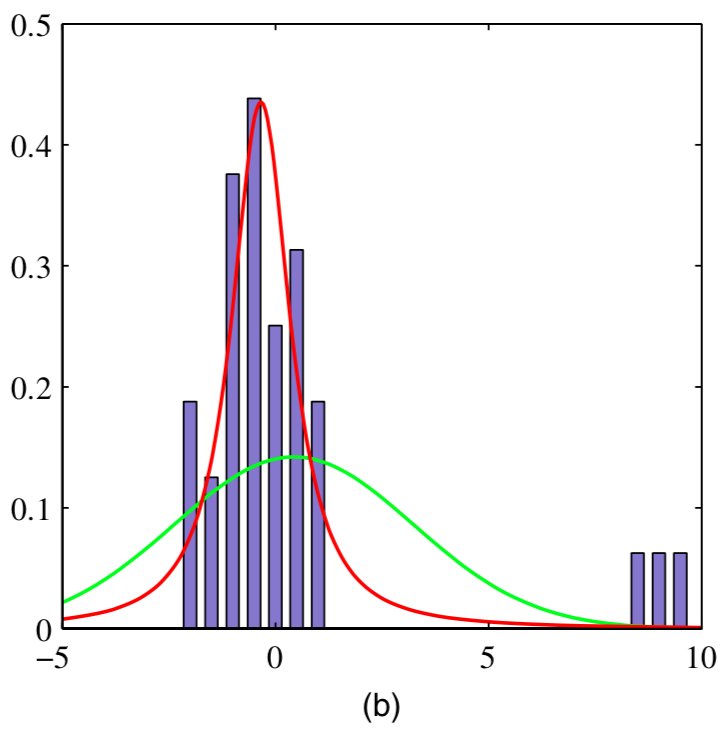
\includegraphics[width = \linewidth]{figure/fig2-16-2.png}     
     \caption{Illustration of robustness of Student's t-distribution compared to a Gaussian. (a) Histogram distribution of 30 data points drawn from a Gaussian distribution, together with the maximum likelihood fit obtained from a t-distribution (red curve) and a Gaussian (green curve, largely hidden by the red curve). Because the t-distribution contains the Gaussian as a special case it gives almost the same solution as the Gaussian. (b) The same data set but with three additional outlying data points showing how the Gaussian (green curve) is strongly distorted by the outliers, whereas the t-distribution (red curve) is relatively unaffected.}
     \label{fig:2.16}
\end{figure}

Note that the maximum likelihood solution for the t-distribution can be found using the expectation-maximization (EM) algorithm. Outliers can arise in practical applications either because the process that generates the data corresponds to a distribution having a heavy tail or simply through mislabelled data. The least squares approach to regression does not exhibit robustness, because it corresponds to maximum likelihood under a (conditional) Gaussian distribution. By basing a regression model on a heavy-tailed distribution such as t-distribution, we obtain a more robust model.


\subsection{Mixtures of Gaussians}

In Figure~\ref{fig:2.22} we see that a linear combination of Gaussians can give rise to very complex densities. By using a sufficient number of Gaussians, ans by adjusting their means and covariances as well as the coefficients in the linear combination, almost any continuous density can be approximated to arbitrary accuracy.

\begin{figure}
     \centering
     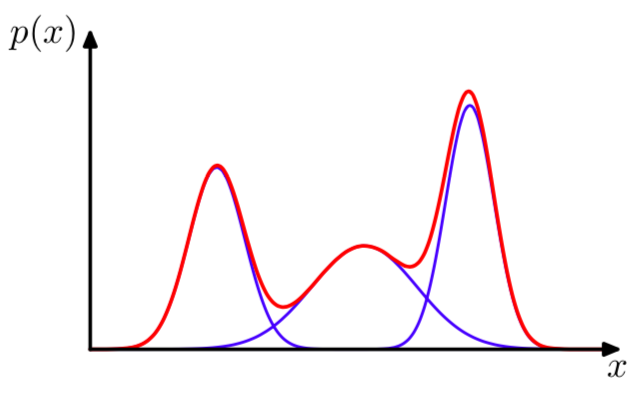
\includegraphics[width = \linewidth]{figure/fig2-22.png}
     \caption{Example of a Gaussian mixture distribution in one dimension showing three Gaussians (each scaled by a coefficient) in blue and their sum in red.}
     \label{fig:2.22}
\end{figure}

We therefore consider a superposition of K Gaussian densities of the form
\begin{equation}
p(\mathbf{x})=\sum_{k=1}^{K} \pi_{k} \mathcal{N}\left(\mathbf{x} | \boldsymbol{\mu}_{k}, \mathbf{\Sigma}_{k}\right)
\end{equation}
which is called a \textit{mixture of Gaussians}. Each Gaussian density $\mathcal{N}(\mathbf{x} | \boldsymbol{\mu}_{k}, \mathbf{\Sigma}_{k})$ is called a \textit{component} of the mixture and has its own mean $\boldsymbol{\mu}_{k}$ and $\mathbf{\Sigma}_{k}$. The parameters $\pi_k$ are called \textit{mixing coefficients}.
\begin{equation}
\begin{aligned} \sum_{k=1}^{K} \pi_{k} &=1 , &  \\ 0 \leqslant \pi_{k} & \leqslant 1 \end{aligned}
\end{equation}

From the sum and product rules, the marginal density is given by 
\begin{equation}
p(\mathbf{x})=\sum_{k=1}^{K} p(k) p(\mathbf{x} | k)
\end{equation}
we can view $\pi_k = p(k)$ as the prior probability of picking the $k^{th}$ component, and the density $\mathcal{N}(\mathbf{x} | \boldsymbol{\mu}_{k}, \mathbf{\Sigma}_{k}) = p(\mathbf{x} | k)$ as the probability of $\boldsymbol{x}$ conditioned on k.



\section{The Exponential Family}

The \textit{exponential family} of distributions over $\boldsymbol{x}$, given parameters $\boldsymbol{\eta}$, is defined to be set of distributions of the form
\begin{equation}
p(\mathbf{x} | \boldsymbol{\eta})=h(\mathbf{x}) g(\boldsymbol{\eta}) \exp \left\{\boldsymbol{\eta}^{\mathrm{T}} \mathbf{u}(\mathbf{x})\right\}
\end{equation}
where $\boldsymbol{x}$ may be scalar or vector, and may be discrete or continuous. Here $\boldsymbol{\eta}$ are called \textit{natural parameters} of the distribution, and $\mathbf{u}(\mathbf{x})$ is some function of $\mathbf{x}$. The function $g(\mathbf{\eta})$ can be interpreted as the coefficient that ensures that the distribution is normalized and therefore satisfies
\begin{equation}
g(\boldsymbol{\eta}) \int h(\mathbf{x}) \exp \left\{\boldsymbol{\eta}^{\mathrm{T}} \mathbf{u}(\mathbf{x})\right\} \mathrm{d} \mathbf{x}=1
\end{equation}
where the integration is replaced by summation if $\mathbf{x}$ is a discrete variable.

Consider first the Bernoulli distribution
\begin{equation}
p(x | \mu)=\operatorname{Bern}(x | \mu)=\mu^{x}(1-\mu)^{1-x}
\end{equation}
which $\mu=\sigma(\eta)$, $\sigma$ is the logistic sigmoid function.
\begin{equation}
p(x | \eta)=\sigma(-\eta) \exp (\eta x)
\end{equation}
\begin{equation}
\begin{aligned} u(x) &=x \\ h(x) &=1 \\ g(\eta) &=\sigma(-\eta) \end{aligned}
\end{equation}

Next consider the multinomial distribution
\begin{equation}
p(\mathbf{x} | \boldsymbol{\mu})=\prod_{k=1}^{M} \mu_{k}^{x_{k}}=\exp \left\{\sum_{k=1}^{M} x_{k} \ln \mu_{k}\right\}
\end{equation}
where $\mathbf{x} = (x_1, \ldots, x_N)^T$, $\eta_k = \ln{\mu_k}$, $\boldsymbol{\eta} = (\eta_1, \ldots, \eta_M)^T$.
\begin{equation}
p(\mathbf{x} | \boldsymbol{\eta})=\exp \left(\boldsymbol{\eta}^{\mathrm{T}} \mathbf{x}\right)
\end{equation}
Note that the parameters $\eta_k$ are not independent because the parameters $\mu_k$ are subject to the constraint
\begin{equation}
\sum_{k=1}^{M} \mu_{k}=1
\end{equation}
\begin{equation}
\begin{aligned}{\exp \left\{\sum_{k=1}^{M} x_{k} \ln \mu_{k}\right\}} \\ {=\exp \left\{\sum_{k=1}^{M-1} x_{k} \ln \mu_{k}+\left(1-\sum_{k=1}^{M-1} x_{k}\right) \ln \left(1-\sum_{k=1}^{M-1} \mu_{k}\right)\right\}} \\ {=\exp \left\{\sum_{k=1}^{M-1} x_{k} \ln \left(\frac{\mu_{k}}{1-\sum_{j=1}^{M-1} \mu_{j}}\right)+\ln \left(1-\sum_{k=1}^{M-1} \mu_{k}\right)\right\}}\end{aligned}
\end{equation}

\begin{equation}
\begin{aligned} \ln \left(\frac{\mu_{k}}{1-\sum_{j} \mu_{j}}\right) =\eta_{k} \\ \mu_{k} =\frac{\exp \left(\eta_{k}\right)}{1+\sum_{j} \exp \left(\eta_{j}\right)} \end{aligned}
\end{equation}
which is called the \textit{softmax} function.
\begin{equation}
p(\mathbf{x} | \boldsymbol{\eta})=\left(1+\sum_{k=1}^{M-1} \exp \left(\eta_{k}\right)\right)^{-1} \exp \left(\boldsymbol{\eta}^{\mathrm{T}} \mathbf{x}\right)   
\end{equation}
This is the standard form of the exponential family, with parameter vector $\boldsymbol{\eta} = (\eta_1, \ldots, \eta_{M-1})^T$ in which
\begin{equation}
\begin{aligned}
\mathbf{u}(\mathbf{x}) &=\mathbf{x} \\ h(\mathbf{x}) &=1 \\ g(\boldsymbol{\eta}) &=\left(1+\sum_{k=1}^{M-1} \exp \left(\eta_{k}\right)\right)^{-1} 
\end{aligned}
\end{equation}

\section{Nonparametric Methods}

The probability distributions having specific functional forms are governed by a small number of parameters whose values are to be determined from a data set. This is called the \textit{parametric} approach to density modelling. An important limitation of this approach is that the chosen density might be a poor model of the distribution that generates the data.

Here, we consider some \textit{nonparametric} approaches to density estimation that make few assumptions about the form of the distribution. Let us start with a discussion of histogram methods for density estimation. 

Given a single continuous variable x, standard histograms simply partition x into distinct bins of width $\Delta$ and then count the number $n_i$ of observations of x falling in bin $i$. 
\begin{equation}
p_{i}=\frac{n_{i}}{N \Delta}
\end{equation}
for which it is easily seen that $\int p(x) \mathrm{d} x=1$. This gives a model for the density $p(x)$ that is constant over the width of each bin.

\begin{figure}
     \centering
     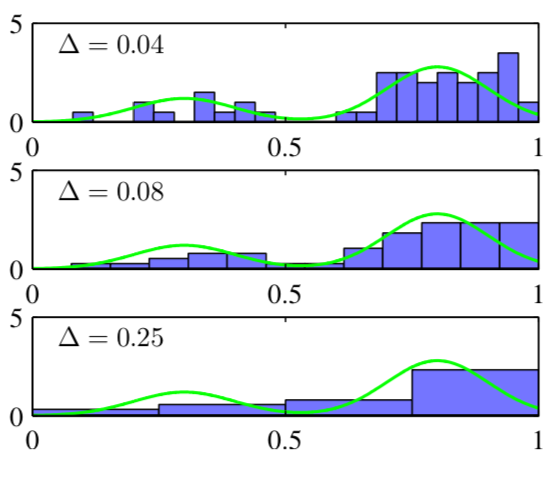
\includegraphics[width = \linewidth]{figure/fig2-24.png}
     \caption{An illustration of the histogram approach to density estimation, in which a data set of 50 data points is generated from the distribution shown by the green curve, which is formed from a mixture of two Gaussians.}
     \label{fig:2.24}
\end{figure}

In Figure~\ref{fig:2.24}, we see that when $\Delta$ is very small (top figure), the resulting density model is very spiky, with a lot of structure that is not present in the underlying distribution that generated the data set. If $\Delta$ is too large (bottom figure) then the result is a model that is too smooth and that consequently fails to capture the bimodal property of the green curve. The best results are obtained for some intermediate value of $\Delta$ (middle figure).

Note that the histogram method has the property that, once the histogram has been computed, the data set itself can be discarded, which can be advantageous if the data set is large. Also the histogram approach is easily applied if the data points are arriving sequentially.


\section*{References}
\bibliography{references}

\begin{thebibliography}{9}

\bibitem{Bishop} 
Bishop, Christopher M. Pattern recognition and machine learning. springer, 2006.

\bibitem{zhengqigao}
https://github.com/zhengqigao/PRML-Solution-Manual


\end{thebibliography}
\end{document}